\let\negmedspace\undefined
\let\negthickspace\undefined
\documentclass[journal]{IEEEtran}
\usepackage[a5paper, margin=10mm, onecolumn]{geometry}
%\usepackage{lmodern} % Ensure lmodern is loaded for pdflatex
\usepackage{tfrupee} % Include tfrupee package

\setlength{\headheight}{1cm} % Set the height of the header box
\setlength{\headsep}{0mm}     % Set the distance between the header box and the top of the text

\usepackage{gvv-book}
\usepackage{gvv}
\usepackage{cite}
\usepackage{amsmath,amssymb,amsfonts,amsthm}
\usepackage{algorithmic}
\usepackage{graphicx}
\usepackage{textcomp}
\usepackage{xcolor}
\usepackage{txfonts}
\usepackage{listings}
\usepackage{enumitem}
\usepackage{mathtools}
\usepackage{gensymb}
\usepackage{comment}
\usepackage[breaklinks=true]{hyperref}
\usepackage{tkz-euclide} 
\usepackage{listings}
% \usepackage{gvv}                                        
\def\inputGnumericTable{}                                 
\usepackage[latin1]{inputenc}                                
\usepackage{color}                                            
\usepackage{array}                                            
\usepackage{longtable}                                       
\usepackage{calc}                                             
\usepackage{multirow}                                         
\usepackage{hhline}                                           
\usepackage{ifthen}                                           
\usepackage{lscape}
\usepackage{circuitikz}
\tikzstyle{block} = [rectangle, draw, fill=blue!20, 
    text width=4em, text centered, rounded corners, minimum height=3em]
\tikzstyle{sum} = [draw, fill=blue!10, circle, minimum size=1cm, node distance=1.5cm]
\tikzstyle{input} = [coordinate]
\tikzstyle{output} = [coordinate]


\begin{document}

\bibliographystyle{IEEEtran}
\vspace{3cm}

\title{1.4.25}
\author{EE25BTECH11009-Anshu kumar ram}
 \maketitle
% \newpage
% \bigskip
{\let\newpage\relax\maketitle}

\renewcommand{\thefigure}{\theenumi}
\renewcommand{\thetable}{\theenumi}
\setlength{\intextsep}{10pt} % Space between text and floats


\numberwithin{equation}{enumi}
\numberwithin{figure}{enumi}
\renewcommand{\thetable}{\theenumi}

\textbf{Question}:\\
Find the position vector of a point $\vec{R}$ which divides the line joining two points $\vec{P}$ and $\vec{Q}$ whose position vectors are $2\vec{a} + \vec{b}$ and $\vec{a} - 3\vec{b}$ externally in the ratio $1:2$.  

\solution \\

The given position vectors are
\begin{align}
    \vec{P} &= 2\vec{a} + \vec{b}, \\
    \vec{Q} &= \vec{a} - 3\vec{b}.
\end{align}


\begin{align}
    \myvec{\vec{P} & \vec{Q}}
    &= \myvec{\vec{a} & \vec{b}}
       \myvec{2 & 1 \\ 1 & -3}
\end{align}

Now, for external division of $\vec{P}\vec{Q}$ in the ratio $1:2$,  
the point $\vec{R}$ is given by
\begin{align}
    \vec{R} &= \frac{1\vec{Q} - 2\vec{P}}{1-2}
\end{align}
\begin{align}
    \vec{R}
    &= \myvec{\vec{P} & \vec{Q}}
       \myvec{-2 \\ 1} \cdot \frac{1}{-1}
\end{align}

Substituting $\myvec{\vec{P} & \vec{Q}}$ in terms of $\vec{a},\vec{b}$:
\begin{align}
    \vec{R}
    &= \myvec{\vec{a} & \vec{b}}
       \myvec{2 & 1 \\ 1 & -3}
       \myvec{-2 \\ 1}\cdot \frac{1}{-1}
\end{align}



\begin{align}
    \therefore \vec{R}
    &= \frac{1}{-1}
       \myvec{\vec{a} & \vec{b}}
       \myvec{-3 \\ -5} \\
    &= \myvec{\vec{a} & \vec{b}}
       \myvec{3 \\ 5}
\end{align}

\newpage

From the figure, it is verified that the theoretical result matches the computational solution.  

\begin{figure}[h!]
    \centering
    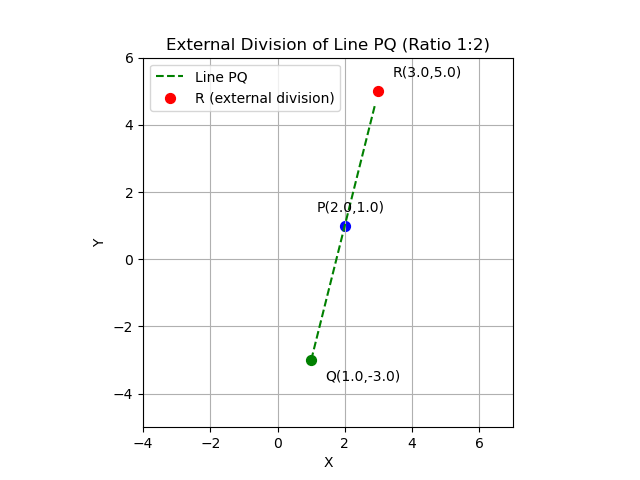
\includegraphics[width=\columnwidth, keepaspectratio]{figs/section_graph.png}
    \label{fig:section_graph}
\end{figure}

\end{document}
